\documentclass[a4paper,11pt,uplatex, titlepage]{jsarticle}
\usepackage{amsmath,amssymb}
\usepackage{bm}
\usepackage[dvipdfmx]{graphicx}
\usepackage{here}
\usepackage{listings,jlisting}

%テキストの表示領域の調節
\setlength{\textwidth}{\paperwidth}
\addtolength{\textwidth}{-40truemm}
\setlength{\textheight}{\paperheight}
\addtolength{\textheight}{-45truemm}

%余白の調節
\setlength{\topmargin}{-10.4truemm}
\setlength{\evensidemargin}{-5.4truemm}
\setlength{\oddsidemargin}{-5.4truemm}
\setlength{\headheight}{17pt}
\setlength{\headsep}{10mm}
\addtolength{\headsep}{-17pt}
\setlength{\footskip}{5mm}

\title{6.画像処理の基礎}
\author{1610004 青木 良太}
\date{提出日 2018年7月19日} % 省略可
\nofiles
\begin{document}
\maketitle

\section{目的}
画像処理は工学の様々な分野で用いられており, 機械系技術者にとっても避けては通れない技術である.
最近は画像処理のパッケージ・ソフトウェアも一般的となり, 様々な処理が手軽に行えるようになっている.
しかし, 自らが新たなシステムを開発する場合はもちろん, 既成のソフトウェアを利用するときにおいても,
処理内容の意味を正しく理解した上で使うことが大切である. 今回の実験では, いくつかの簡単なデジタル画像処理をコンピュータ上で行い,
その基本原理と特性を理解することを目的とする.
\section{理論}
\subsubsection{画像処理}
画像処理(image processing)とは画像で表現された情報の処理の総称であり, 図\ref{contents}に示すように様々な内容が含まれる.
ただし, 狭義には, 2次元画像を処理して新たな2次元画像を生成したり, 画像から何らかの情報取り出したりすること意味し,
歪の修正, ぼけやノイズの除去, 特定成分の強調などの画像変換やパターンを挿す場合も多い. 画像処理にコンピュータを利用すると便利なことが多いが,
決して必須ではない. 例えば, 写真の現像は化学的方法によって, 偏光フィルタによる成分抽出は光学的方法によって行われる.
また, 種々の処理を専用の電子回路によって行うことも可能であるし, 生物が非常に高度な画像処理を瞬時に行なっていることは言うまでもない.

\begin{figure}[H]
  \begin{center}
    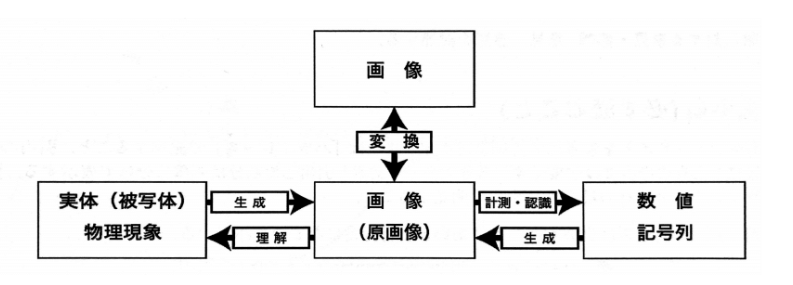
\includegraphics[width = 5cm]{pic/contents.png}
    \caption{画像処理の内容}
    \label{contents}
  \end{center}
\end{figure}

\subsubsection{画像のディジタル化}
現在一般に使われているノイマン型のコンピュータは, 自然界に存在する連続量をそのままの形で取り扱うことができない.
そこで, コンピュータで画像処理を行う場合, 画像を標本化(sampling)と量子化(quantization)と言う二つのプロセスによって離散化し,
ディジタル(digital)量として表現する. 標本化とは時間的あるいは空間的に連続して変化する信号から,
その軸上のいくつかの離散点における値を取り出す操作のことで, 画像情報においては画面を正方形や六角形などの画素(pixel)に区切ることで実現される.
また, 量子化は各画素内の明るさを代表する値を階調値(gray level)と呼ばれる有限個のレベルのどれかに割り当てることで実現される.
これらの操作によって表現された画像をディジタル画像(digital image)という. すなわち, ディジタル画像とは図に示すように,
明るさに対応した離散量をもつ有限個の画素2次元に集まって構成された画像のことである.
ディジタル画像は階調値の取る個数(階調数)によって表1のように分類することができる.

\begin{table}[H]
  \begin{center}
    \caption{ディジタル画像の種類}
    \begin{tabular}{|l|l|}
    \hline
    二値画像 & 階調値が0(黒)または1(白)の画像 \\ \hline
    濃淡画像 & 階調値が2より大きい画像  \\ \hline
    カラー画像 & 三原色でそれぞれに対して階調数が2より大きい画像 \\ \hline
    \end{tabular}
  \end{center}
\end{table}

\subsection{画像演算}
一つのディジタル画像に何らかの処理を施して別の画像を得ることを, 画像演算という.
今, ディジタル画像全体の集合を$D$,$D$の部分集合を$D_1,D_2,D_3$と書けば, 画像 $F \in D_1, G \in D_2, H \in D_3$
に対して,
\begin{align}
  G = O(F) \\
  H = \Phi(F,G)
\end{align}
という演算を考えることができる. 式(1)における写像$O: D_1 \to D_2$を単項演算, 式(2)における写像$\Phi: D_1 \times D_2 \to D_3$
を二項演算という. 画像二項演算には実数演算と同様に, 論理演算, 四則演算, Max/Min演算が定義される.
\subsection{フィルタリング}
画像のフィルタリング(filterling)とは, 任意の画素の新しい階調値を注目画素の近傍(neighborhood)内に
ある画素の階調値から決定する局所演算(local operation)を画像上のすべての画素に対して行う処理のことである.
このとき, 各画素に対する演算はその位置によらず独立して行われ, 近傍の範囲は画像全体に比べて十分小さい. このような近傍は範囲をマスクと呼び,
フィルタリングにおいては$3\times3, 5\times5, 7\times7$などのマスクが適用される. フィルタリングは画像認識などの前処理として用いられることが多い.
\subsubsection{平滑化フィルタ}
注目画素の近傍内にある画素の階調値の平均値を求め, それを注目がその新しい階調値にすることを考える. 新しい画像を$G = g(i,j)$とすると, 求める式は次のように表される.
\begin{align}
  g(i,j) = \frac{1}{9} \sum_{m=-1}^{1} \sum_{n=-1}^{1} f(i+m, j+n)
\end{align}
このような演算を行うフィルタは, 画像中の階調値の変化を滑らかにしてノイズを除去する機能を持つことから平滑化フィルタと呼ばれる. フィルタは演算に用いる
係数をマトリクス状に並べて表示することができる. 例えば, 式(3)のフィルタは図\ref{heikatsuka}に示されるような$3\times3$マスクに
よって表される. なお, 図\ref{omomi}のように注目画素の重みを大きくした平滑化フィルタも存在する. 図\ref{omomi}のフィルタを数式で表すと,
式(4)のようになる.
\begin{align}
  g(i,j) = \frac{1}{10} { \sum_{m=-1}^{1} \sum_{n=-1}^{1} f(i+m, j+n)+f(i,j) }
\end{align}

\begin{figure}[H]
  \begin{tabular}{cc}
    \begin{minipage}{0.5\hsize}
      \begin{center}
      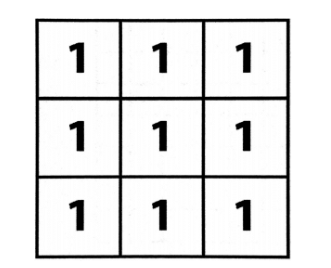
\includegraphics[width = 5cm]{pic/heikatsuka.png}
      \caption{平滑化フィルタ}
      \label{heikatsuka}
      \end{center}
    \end{minipage}

    \begin{minipage}{0.5\hsize}
      \begin{center}
        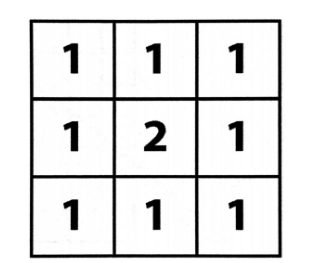
\includegraphics[width = 5cm]{pic/omomi.png}
        \caption{平滑化フィルタ(重み2)}
        \label{omomi}
      \end{center}
    \end{minipage}
  \end{tabular}
\end{figure}

\subsubsection{差分型フィルタ}
差分型フィルタ(difficult filter)は, 注目画素の近傍の階調値の微分(差分)をとるフィルタで,
画像中の線や縁など階調変化の急な部分を抽出することができる. 例として, 水平方向の微分$\partial f / \partial j$は$3\times3$
マスクを用いれば,
\begin{align}
  g(i,j)=-f(i-1,j-1)+f(i+1,j-1)-f(i-1,j)+f(i+1,j)-f(i-1,j+1)+(i+1,j+1)
\end{align}
のように求められる. 同様の手順により, 垂直方向の微分$\partial f / \partial j$を表す$3\times3$マスクのフィルタを得ることができる.
\subsubsection{ラプラシアンフィルタ}
二次の空間微分であるラプラシアン(Laplacian)
\begin{align}
  \Delta = \nabla^{2} = \frac{\partial^{2}}{\partial j^{2}}
\end{align}
は, 画像中の輪郭線の長さを強調する機能を持っている. これをフィルタとして用いたものがラプラシアンフィルタであり,
$3\times3$マスクを用いた4近傍に対するラプラシアンフィルタは図のように表される.
\subsection{点演算}
画像中のある領域の画素の階調値を問題にする時, 注目画素における階調値をそのまま用いるのではなく,
何らかの変換を行った値を用いたほうが便利なことがある. 点演算(point operation)はこのような場合に行われる処理で,
新しい画像上の画素の階調値を元の画像の同じ位置における階調値から決定するものである.
\subsubsection{二値化}
設定したしきい値(threshold level)よりも小さい階調値を持つ画素を0(黒), 大きい階調値を持つ画素を
1(白)にすることで, 階調画像を二値画像に変換する処理のことを二値化(binarization)という.
しきい値には, 濃度ヒストグラム(横軸に階調値, 縦軸に画素数をとったグラフ)の谷部分や, 二分割される画素数が適当な割合になる位置などが選ばれるが,
結果に大きな影響を与えるので注意する.
\subsubsection{階調変換}
適当な関数を定義することで, 画像中の階調値の分布範囲や分布関数を目的のものに変える処理が階調変換(gray level conversion)である.
例えば, 階調値$L$がある狭い範囲$[L_1,L_2]$にしか分布していない画像は, コントラストが不明瞭になっていることが多い.
このような場合, 原画像に次式で定義される線形変換を施して階調変化の範囲を$[L_{min},L_{max}]$まで広げれば, 画像のコントラストを明瞭にすることができる.
\begin{align}
  L^{*} = \frac{L_{max}-L_{min}}{L_2-L_1}(L-L_1)+L_{min}
\end{align}
ここで, $L^{*}$は変換後の階調値である.

\section{実験方法}
\subsection{課題1: 画素値と画像の関係}
この課題は画素値による色調の変化を確かめることを目的とした.
真っ黒の画像(hoge)を指定した画素値に変換するソースコードを画素値を70,150,200に変化させて, 実行した.
以下に実行したソースコードの一部を示す.

\begin{lstlisting}[basicstyle=\ttfamily\footnotesize]
# 真っ黒の画像を生成
gazo = zeros( (10,10) )

# 画像を変換
for x in range(10):
  for y in range(10):
      gazo[y][x] = 200 #この値を70,150,200と変化させた.
\end{lstlisting}

\subsection{課題2: 画素位置と画像の関係}
この課題では, 画素位置を指定することで画像がどのように変化するかを調べることを目的とした.
真っ黒な画像に画素位置([0][0],[0][0],[0][9],[9][0])を指定し,その対応と変化を確認した.
以下に実行したソースコードの一部を示す.

\begin{lstlisting}[basicstyle=\ttfamily\footnotesize]
# 真っ黒の画像を生成
gazo = zeros( (10,10) )

gazo[3][7] = 255 #[3][7]を[0][0],[0][9],[9][0]に変化させた.
\end{lstlisting}

\subsection{課題3: 図形の描画}
この課題では, 課題1と課題2で確認した画素位置や画素値と画像の関係を用いて図形を描画することを目的とした.
真っ黒な画像を変換して白い正方形が中央に表示されるようにプログラムを書いた.
以下に実行したソースコードの一部を示す.
\begin{lstlisting}[basicstyle=\ttfamily\footnotesize]
# 真っ黒の画像を生成
gazo = zeros( (10,10) )

# 画像を変換
for x in range(10):
    for y in range(10):
        if (x<=8 and x>=1) and (y<=8 and y>=1) :
            gazo[y][x] = 255
\end{lstlisting}

\subsection{課題4: フィルタ}
この課題では移動平均フィルタ, ラプラシアンフィルタを用いることで実際にどのような効果があるのか確認することを目的とした.
フィルタの値を変え, 以下に示す移動平均フィルタ, ラプラシアンフィルタを実装した.
以下に実行したソースコードの一部を示す.

\begin{lstlisting}[basicstyle=\ttfamily\footnotesize]
# 画像を読み込み
gazo = imread( "kadai4.bmp", 0 )

gazo2 = zeros((12,12))
#移動平均フィルタの場合##################################################
for x in range(1,11):
    for y in range(1,11):
        filter = [
              [1, 1, 1],  
              [1, 1, 1],
              [1, 1, 1]
              ]

        gasochi = 0
        for xx in range(3):
            for yy in range(3):
                # ここでfilterの値をgazoに掛ける
                gasochi += gazo[y+yy-1][x+xx-1] * filter[yy][xx]
                gasochi /= 9

#ラプラシアンフィルタの場合###############################################
for x in range(1,11):
    for y in range(1,11):
        filter = [
            [0, 1, 0],  
            [1, -4, 1],
            [0, 1, 0]
            ]

        gasochi = 0
        for xx in range(3):
            for yy in range(3):
                # ここでfilterの値をgazoに掛ける
                gasochi += gazo[y+yy-1][x+xx-1] * filter[yy][xx]
#####################################################################

        # 0〜255の範囲内に収める
        gasochi = int(gasochi)
        if gasochi<0:
            gasochi = 0
        elif gasochi>255:
            gasochi = 255
        gazo2[y][x] = gasochi
\end{lstlisting}

\subsection{課題5: ヒストグラムと二値化}
この課題では, 画素値を表示するヒストグラムを参照して, 画像の特徴を表す二値画像を生成することで
画像を見やすく処理することを目的とした.
表示されるヒストグラムから閾値を決定し, その閾値を境として0と255のみを画素値として指定することで実装を行なった.
以下にヒストグラムと実行したソースコードの一部を示す.

\begin{figure}[H]
  \begin{center}
    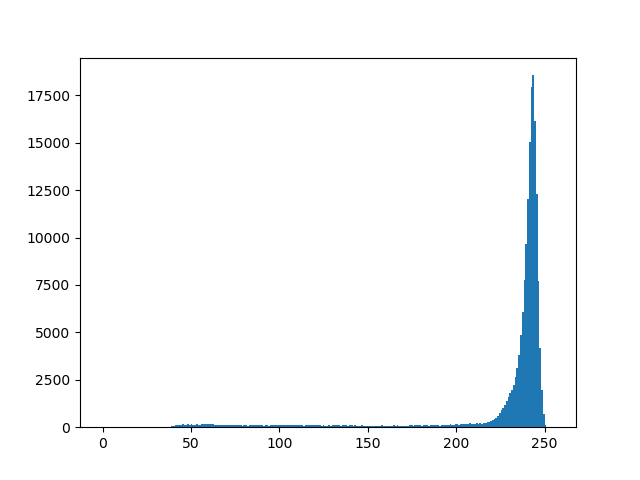
\includegraphics[width = 5cm]{pic/kadai5_graph1.png}
    \caption{二値化処理を施す画像から得られたヒストグラム}
    \label{5_hist}
  \end{center}
\end{figure}

\begin{lstlisting}[basicstyle=\ttfamily\footnotesize]
# 画像を読み込み
gazo = imread( "kadai5.bmp", 0 )

# ヒストグラムを表示
figure()
hist( gazo.flatten(), 256, (0,255) )

# 画像を変換
gazo2 = zeros((396,455))
for x in range(455):
    for y in range(396):

        if gazo[y][x]<200:
            gazo2[y][x] = 0
        else:
            gazo2[y][x] = 255
\end{lstlisting}

\subsection{課題6: ヒストグラムと階調変換}
この課題では, 画素値を表示するヒストグラムを参照して, 濃淡がよりはっきりとした画像を生成するようプログラムを実装し,
その効果を確認することを目的とした.
画素値の範囲が狭く, 濃淡がはっきりとしていない画像に対して, 式(7)を用いて階調変換することで濃淡を強調させた.
この時ヒストグラムから, $L_{max} = 255, L_{min} = 0, L_1 = 120, L_2 = 150$として読み取った.
以下に実行したソースコードの一部を示す.
\begin{lstlisting}[basicstyle=\ttfamily\footnotesize]
# 画像を読み込み
gazo = imread( "kadai6.bmp", 0 )

# 画像を変換
gazo2 = zeros((240,384))
for x in range(384):
    for y in range(240):
        gazo2[y][x] = (255*(gazo[y][x]-120)/30) + 0
\end{lstlisting}

\subsection{課題7: 図形の面積の計算}
この課題では課題1〜6で学んだ処理を用いて画像に描かれている画素数の異なる6つの図形の面積をそれぞれ求めることを目的とした.
今回はヒストグラムから6つの画像の画素値を特定し, それぞれの画素値をもつ画素を数え上げるという処理を行った.
以下に使用した画像と実行したソースコードの一部を示す.

\begin{figure}[H]
  \begin{tabular}{cc}
    \begin{minipage}{0.5\hsize}
      \begin{center}
        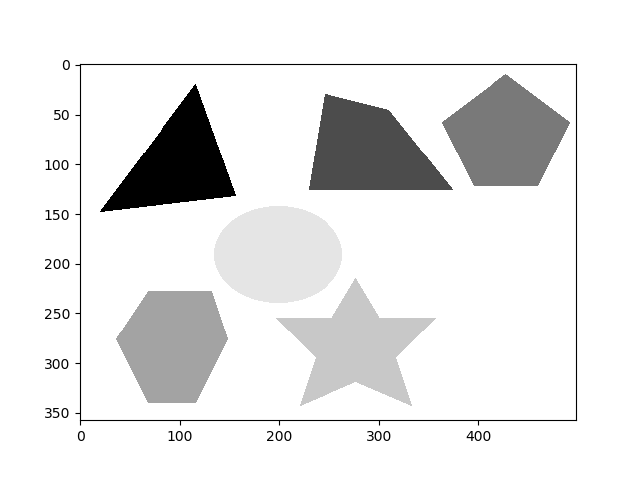
\includegraphics[width = 5cm]{pic/kadai7_1.png}
        \caption{課題で使用した6つの図形}
        \label{7}
      \end{center}
    \end{minipage}

    \begin{minipage}{0.5\hsize}
      \begin{center}
        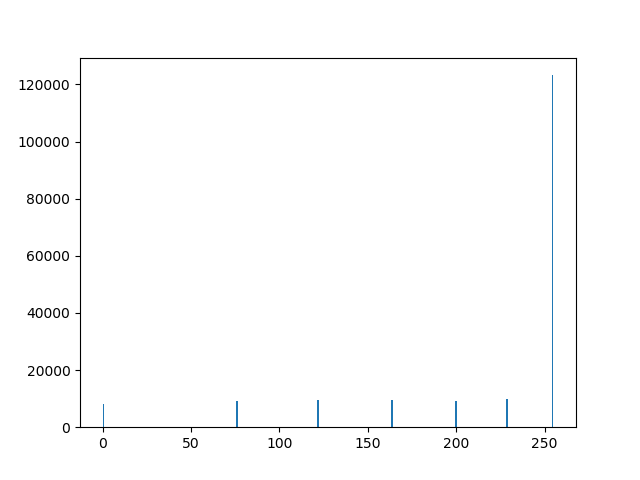
\includegraphics[width = 5cm]{pic/kadai7_2.png}
        \caption{課題で使用した6つの図形のヒストグラム}
        \label{7_hist}
      \end{center}
    \end{minipage}
  \end{tabular}
\end{figure}

\begin{lstlisting}[basicstyle=\ttfamily\footnotesize]
# 画像の読み込み
gazo = imread( "kadai7.bmp", 0 )

a1 = 0 #左上
a2 = 0 #上真ん中
a3 = 0 #右上
a4 = 0 #左下
a5 = 0 #右下
a6 = 0 #真ん中

for y in range(0,358):
    for x in range(0,499):
        if gazo[y][x] == 0:
            a1 += 1
        elif gazo[y][x] ==76:
            a2 += 1
        elif gazo[y][x] == 122:
            a3 += 1
        elif gazo[y][x] == 164:
            a4 += 1
        elif gazo[y][x] == 200:
            a5 += 1
        elif gazo[y][x] == 229:
            a6 += 1

print("三角形の面積:%d"%a1)
print("四角形の面積:%d"%a2)
print("五角形の面積:%d"%a3)
print("六角形の面積:%d"%a4)
print("星形の面積:%d"%a5)
print("楕円の面積:%d"%a6)
\end{lstlisting}

\subsection{課題8: 図形の輪郭線の長さの長さの計算}
この課題では課題1〜6で学んだ処理を用いて画像に描かれている画素数の異なる6つの図形の輪郭線の長さをそれぞれ求めることを目的とした.
ラプラシアンフィルタと二値化を用いて画像の輪郭を強調したのち,
以下に使用した画像とソースコードの一部を示す.

\begin{figure}[H]
    \begin{center}
      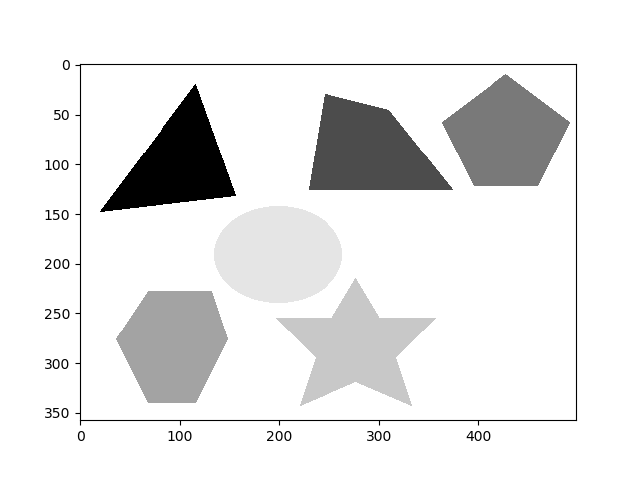
\includegraphics[width = 5cm]{pic/kadai8_1.png}
      \caption{課題で使用した6つの図形}
      \label{8}
      \end{center}
\end{figure}

\begin{lstlisting}[basicstyle=\ttfamily\footnotesize]
# 画像の読み込み
gazo = imread( "kadai8.bmp", 0 )

    c = 0
    gazo2 = zeros( (358,499) )#二値化###################################
    for y in range(1,357):
        for x in range(1,498):
            if gazo[y][x] < 240: #220 200 160 120 50をそれぞれ代入した.
                gazo2[y][x] = 0
            else:
                gazo2[y][x] = 255

    gazo3 = zeros( (358,499) )#ラプラシアンフィルタ#######################
    for y in range(1,357):
        for x in range(1,498):

            filter = [
                [0, 1, 0],
                [1, -4, 1],
                [0, 1, 0]
                ]

            gasochi = 0
            for xx in range(3):
                for yy in range(3):
                    # ここでfilterの値をgazoに掛ける
                    gasochi += gazo2[y+yy-1][x+xx-1] * filter[yy][xx]

            gasochi = int(gasochi)
            if gasochi<0:
                gasochi = 0
            elif gasochi>255:
                gasochi = 255
            gazo3[y][x] = gasochi

    for y in range(0,358):
        for x in range(0,499):
            if gazo3[y][x] == 255:
                c += 1

    print(c)
\end{lstlisting}

\section{実験結果及び考察}
\subsection{課題1: 画素値と画像の関係}
画素値を70,150,200と変化させた時の実行結果を以下に示す.

\begin{figure}[H]
  \begin{tabular}{cc}
    \begin{minipage}{0.5\hsize}
      \begin{center}
        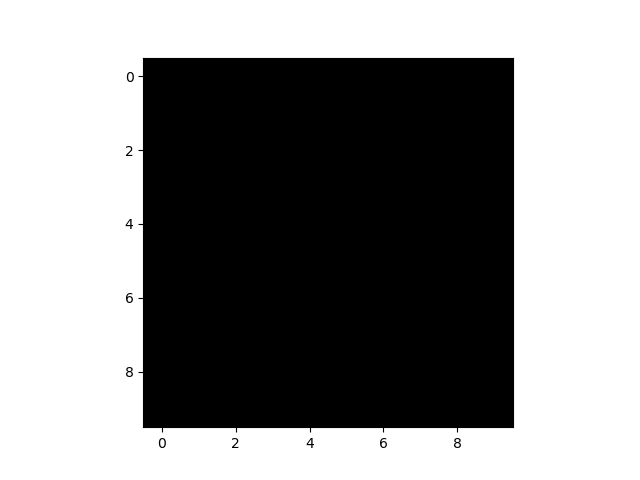
\includegraphics[width = 5cm]{pic/kadai_1.png}
        \caption{変換前(画素値:0)}
        \label{black1}
      \end{center}
    \end{minipage}

    \begin{minipage}{0.5\hsize}
      \begin{center}
        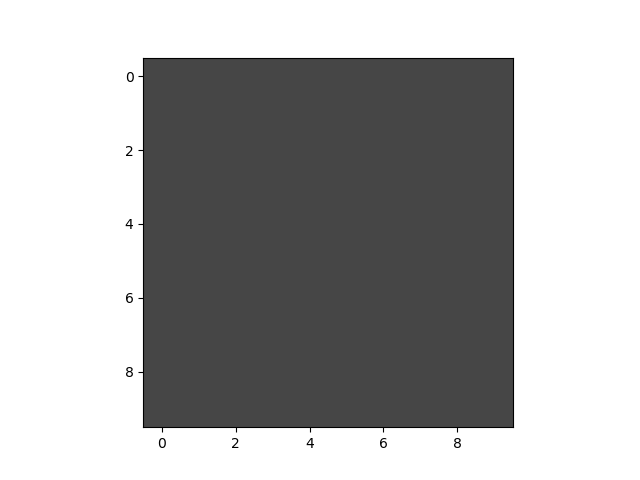
\includegraphics[width = 5cm]{pic/kadai_1_70.png}
        \caption{変換後(画素値:70)}
        \label{1_70}
      \end{center}
    \end{minipage}
  \end{tabular}
\end{figure}

\begin{figure}[H]
  \begin{tabular}{cc}
    \begin{minipage}{0.5\hsize}
      \begin{center}
        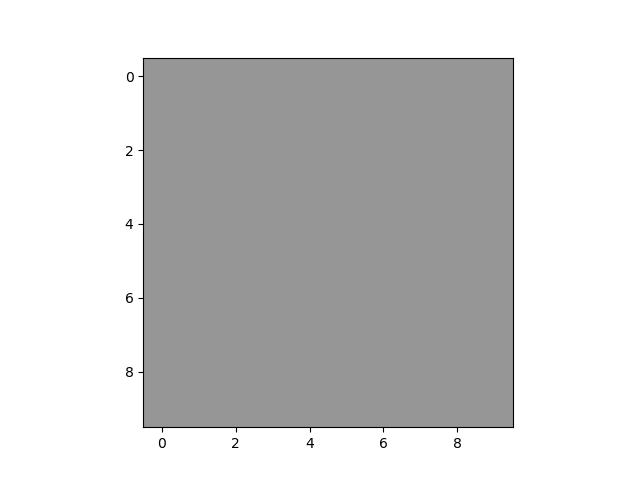
\includegraphics[width = 5cm]{pic/kadai_1_150.png}
        \caption{変換後(画素値:150)}
        \label{1_150}
      \end{center}
    \end{minipage}

    \begin{minipage}{0.5\hsize}
      \begin{center}
        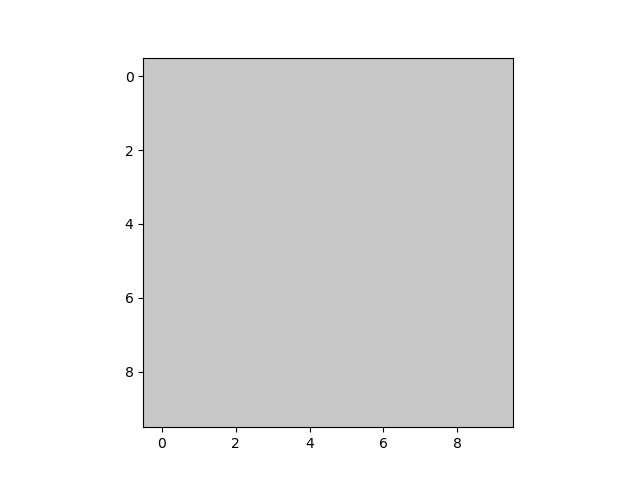
\includegraphics[width = 5cm]{pic/kadai1_200.png}
        \caption{変換後(画素値:200)}
        \label{1_200}
      \end{center}
    \end{minipage}
  \end{tabular}
\end{figure}

図\ref{black1}〜\ref{1_200}を見ると画素値が255に近づくにつれ白くなり, 0に近づくにつれ黒くなっていることがわかる.
ソースコードではgazo[y][x] = 画素値とし, xとyを0から9まで変化することで全ての画素位置に指定した画素値を代入している.

\subsection{課題2: 画素位置と画像の関係}
画素位置を[3][7],[0][0],[0][9],[9][0]と変化させた実行結果を以下に示す.

\begin{figure}[H]
  \begin{tabular}{cc}
    \begin{minipage}{0.5\hsize}
      \begin{center}
        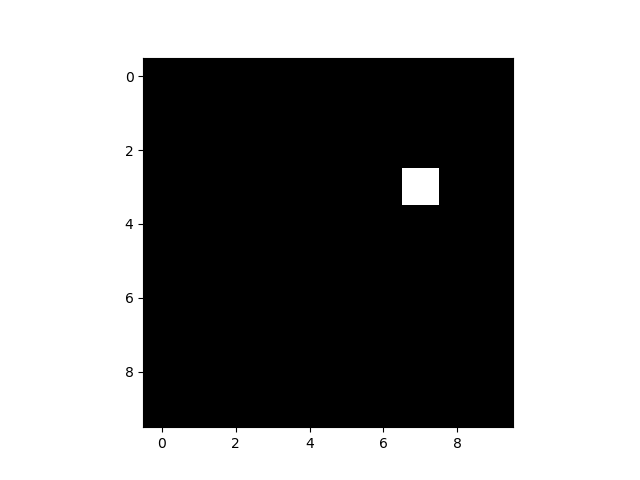
\includegraphics[width = 5cm]{pic/kadai2_37.png}
        \caption{画像位置:[3][7]}
        \label{2_37}
      \end{center}
    \end{minipage}

    \begin{minipage}{0.5\hsize}
      \begin{center}
        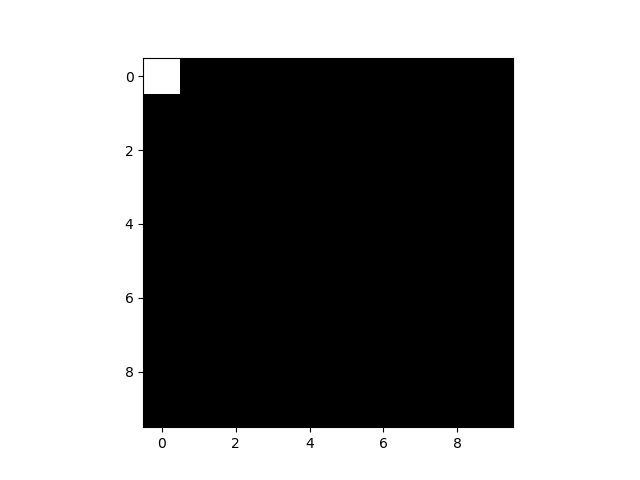
\includegraphics[width = 5cm]{pic/kadai2_00.png}
        \caption{画像位置:[0][0]}
        \label{2_00}
      \end{center}
    \end{minipage}
  \end{tabular}
\end{figure}

\begin{figure}[H]
  \begin{tabular}{cc}
    \begin{minipage}{0.5\hsize}
      \begin{center}
        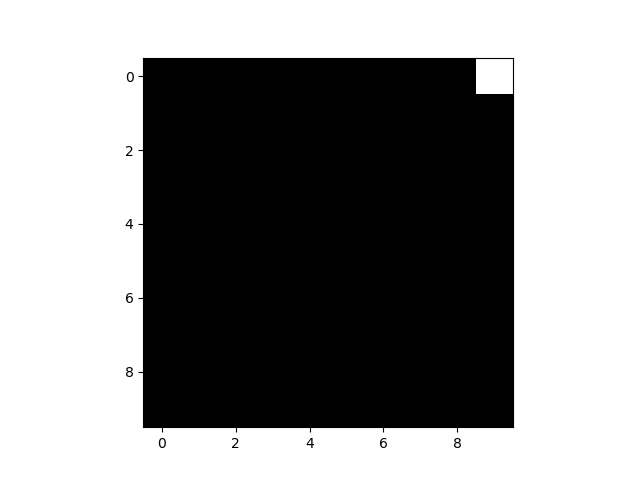
\includegraphics[width = 5cm]{pic/kadai2_09.png}
        \caption{画像位置:[0][9]}
        \label{2_09}
      \end{center}
    \end{minipage}

    \begin{minipage}{0.5\hsize}
      \begin{center}
        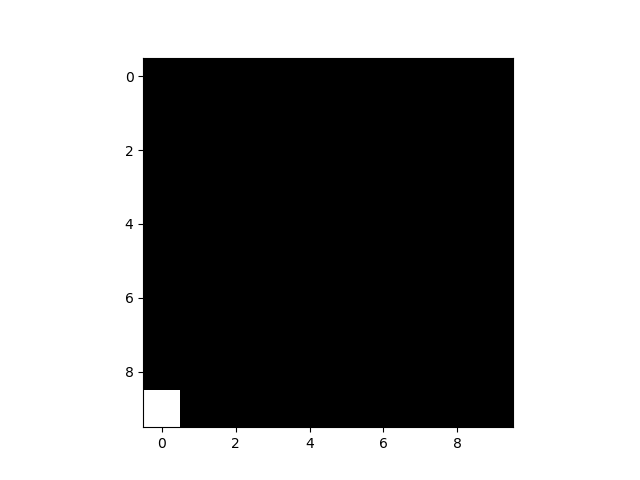
\includegraphics[width = 5cm]{pic/kadai2_90.png}
        \caption{画像位置:[9][0]}
        \label{2_90}
      \end{center}
    \end{minipage}
  \end{tabular}
\end{figure}

\begin{lstlisting}[basicstyle=\ttfamily\footnotesize]
#[3][7]の時
[[  0.   0.   0.   0.   0.   0.   0.   0.   0.   0.]
 [  0.   0.   0.   0.   0.   0.   0.   0.   0.   0.]
 [  0.   0.   0.   0.   0.   0.   0.   0.   0.   0.]
 [  0.   0.   0.   0.   0.   0.   0. 255.   0.   0.]
 [  0.   0.   0.   0.   0.   0.   0.   0.   0.   0.]
 [  0.   0.   0.   0.   0.   0.   0.   0.   0.   0.]
 [  0.   0.   0.   0.   0.   0.   0.   0.   0.   0.]
 [  0.   0.   0.   0.   0.   0.   0.   0.   0.   0.]
 [  0.   0.   0.   0.   0.   0.   0.   0.   0.   0.]
 [  0.   0.   0.   0.   0.   0.   0.   0.   0.   0.]]

#[0][0]の時
[[255.   0.   0.   0.   0.   0.   0.   0.   0.   0.]
 [  0.   0.   0.   0.   0.   0.   0.   0.   0.   0.]
 [  0.   0.   0.   0.   0.   0.   0.   0.   0.   0.]
 [  0.   0.   0.   0.   0.   0.   0.   0.   0.   0.]
 [  0.   0.   0.   0.   0.   0.   0.   0.   0.   0.]
 [  0.   0.   0.   0.   0.   0.   0.   0.   0.   0.]
 [  0.   0.   0.   0.   0.   0.   0.   0.   0.   0.]
 [  0.   0.   0.   0.   0.   0.   0.   0.   0.   0.]
 [  0.   0.   0.   0.   0.   0.   0.   0.   0.   0.]
 [  0.   0.   0.   0.   0.   0.   0.   0.   0.   0.]]

#[0][9]の時
[[  0.   0.   0.   0.   0.   0.   0.   0.   0. 255.]
 [  0.   0.   0.   0.   0.   0.   0.   0.   0.   0.]
 [  0.   0.   0.   0.   0.   0.   0.   0.   0.   0.]
 [  0.   0.   0.   0.   0.   0.   0.   0.   0.   0.]
 [  0.   0.   0.   0.   0.   0.   0.   0.   0.   0.]
 [  0.   0.   0.   0.   0.   0.   0.   0.   0.   0.]
 [  0.   0.   0.   0.   0.   0.   0.   0.   0.   0.]
 [  0.   0.   0.   0.   0.   0.   0.   0.   0.   0.]
 [  0.   0.   0.   0.   0.   0.   0.   0.   0.   0.]
 [  0.   0.   0.   0.   0.   0.   0.   0.   0.   0.]]

#[9][0]の時
[[  0.   0.   0.   0.   0.   0.   0.   0.   0.   0.]
 [  0.   0.   0.   0.   0.   0.   0.   0.   0.   0.]
 [  0.   0.   0.   0.   0.   0.   0.   0.   0.   0.]
 [  0.   0.   0.   0.   0.   0.   0.   0.   0.   0.]
 [  0.   0.   0.   0.   0.   0.   0.   0.   0.   0.]
 [  0.   0.   0.   0.   0.   0.   0.   0.   0.   0.]
 [  0.   0.   0.   0.   0.   0.   0.   0.   0.   0.]
 [  0.   0.   0.   0.   0.   0.   0.   0.   0.   0.]
 [  0.   0.   0.   0.   0.   0.   0.   0.   0.   0.]
 [255.   0.   0.   0.   0.   0.   0.   0.   0.   0.]]
\end{lstlisting}

図\ref{2_37}〜\ref{2_90}から,最初の[]ではx軸の画素位置を表しており, 二番目の[]ではy軸の画素位置を表している.
また,今回の実験では0から9までの範囲がそれぞれ取れることがわかる.つまり,[0][0]から[9][9]までの座標を任意に指定
することで画像の任意の位置の画素を指定することができるのである.ソースコードではこれをgazo[3][7] = 255と記述しており,
画素位置に画素値を代入することで表現している.

\subsection{課題3: 図形の描画}
以下にソースコードの実行結果を示す.

\begin{figure}[H]
  \begin{tabular}{cc}
    \begin{minipage}{0.5\hsize}
      \begin{center}
        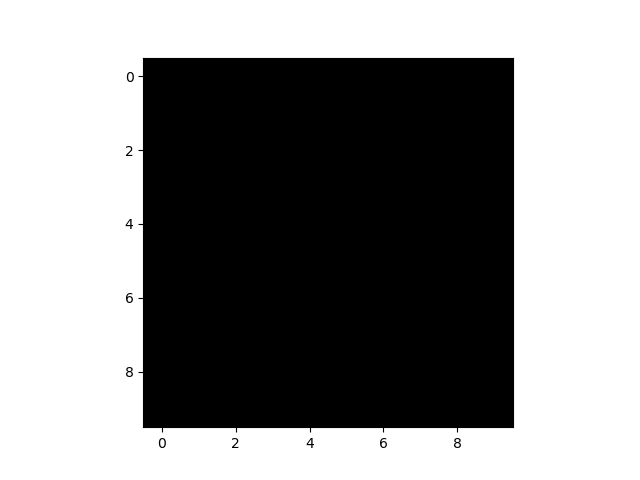
\includegraphics[width = 5cm]{pic/kadai_1.png}
        \caption{変換前の画像}
        \label{black2}
      \end{center}
    \end{minipage}

    \begin{minipage}{0.5\hsize}
      \begin{center}
        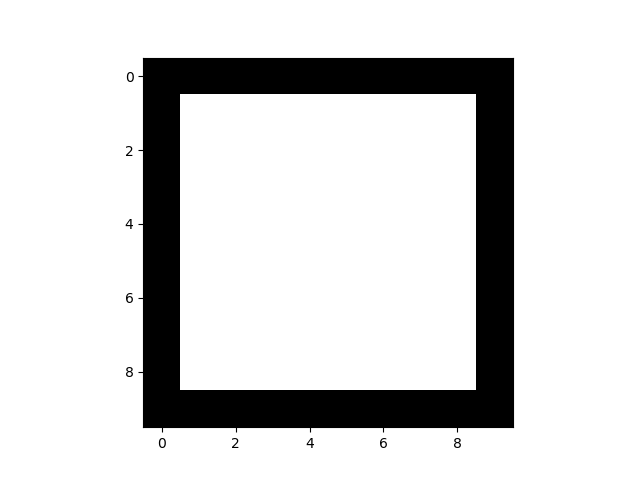
\includegraphics[width = 5cm]{pic/kadai3_success.png}
        \caption{変換後の画像(白い正方形)}
        \label{white_square}
      \end{center}
    \end{minipage}
  \end{tabular}
\end{figure}

\begin{lstlisting}[basicstyle=\ttfamily\footnotesize]
#変換後の画素値
[[  0.   0.   0.   0.   0.   0.   0.   0.   0.   0.]
 [  0. 255. 255. 255. 255. 255. 255. 255. 255.   0.]
 [  0. 255. 255. 255. 255. 255. 255. 255. 255.   0.]
 [  0. 255. 255. 255. 255. 255. 255. 255. 255.   0.]
 [  0. 255. 255. 255. 255. 255. 255. 255. 255.   0.]
 [  0. 255. 255. 255. 255. 255. 255. 255. 255.   0.]
 [  0. 255. 255. 255. 255. 255. 255. 255. 255.   0.]
 [  0. 255. 255. 255. 255. 255. 255. 255. 255.   0.]
 [  0. 255. 255. 255. 255. 255. 255. 255. 255.   0.]
 [  0.   0.   0.   0.   0.   0.   0.   0.   0.   0.]]
\end{lstlisting}

ソースコードでは, x座標が1から8かつy座標が1から8の画素の画素値を255にすることで白い正方形を表現している.
今回行った処理を様々な画素値や範囲指定をすることで様々な図形が描画できると考えられる.

\subsection{課題4: フィルタ}
変換の実行結果を以下に示す.

\begin{figure}[H]
  \begin{center}
    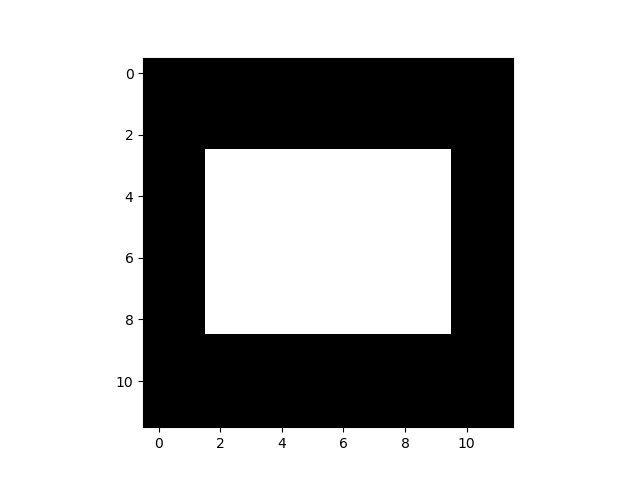
\includegraphics[width = 5cm]{pic/kadai4.png}
    \caption{フィルタ変換前の画像}
    \label{beforefilter}
  \end{center}
\end{figure}

\begin{figure}[H]
  \begin{tabular}{cc}
    \begin{minipage}{0.5\hsize}
      \begin{center}
        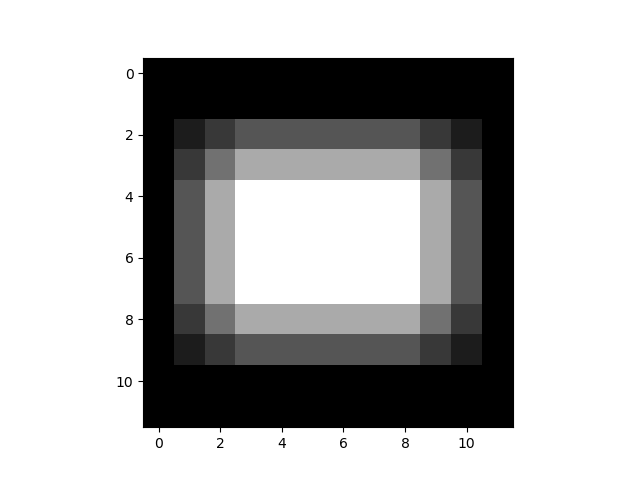
\includegraphics[width = 5cm]{pic/kadai4_1.png}
        \caption{移動平均フィルタ変換後の画像}
        \label{meanfilter}
      \end{center}
    \end{minipage}

    \begin{minipage}{0.5\hsize}
      \begin{center}
        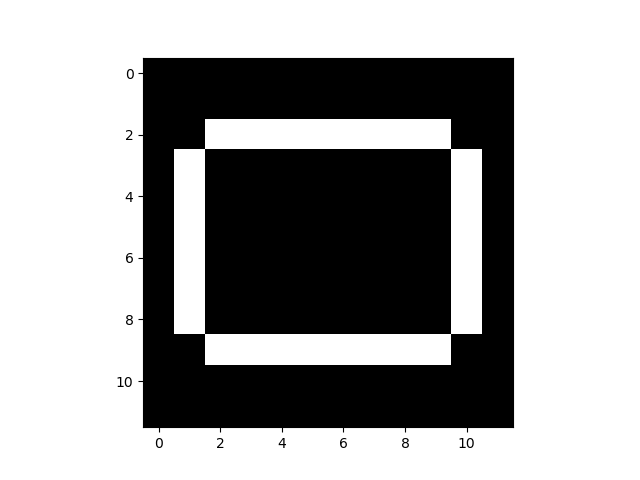
\includegraphics[width = 5cm]{pic/kadai4_raplace.png}
        \caption{ラプラシアンフィルタ変換後の画像}
        \label{raplacefilter}
      \end{center}
    \end{minipage}
  \end{tabular}
\end{figure}

\begin{lstlisting}[basicstyle=\ttfamily\footnotesize]
#変換前の画素値
[[  0   0   0   0   0   0   0   0   0   0   0   0]
 [  0   0   0   0   0   0   0   0   0   0   0   0]
 [  0   0   0   0   0   0   0   0   0   0   0   0]
 [  0   0 255 255 255 255 255 255 255 255   0   0]
 [  0   0 255 255 255 255 255 255 255 255   0   0]
 [  0   0 255 255 255 255 255 255 255 255   0   0]
 [  0   0 255 255 255 255 255 255 255 255   0   0]
 [  0   0 255 255 255 255 255 255 255 255   0   0]
 [  0   0 255 255 255 255 255 255 255 255   0   0]
 [  0   0   0   0   0   0   0   0   0   0   0   0]
 [  0   0   0   0   0   0   0   0   0   0   0   0]
 [  0   0   0   0   0   0   0   0   0   0   0   0]]

 #移動平均フィルタ変換後の画素値
 [  0.   0.   0.   0.   0.   0.   0.   0.   0.   0.   0.   0.]
 [  0.   0.   0.   0.   0.   0.   0.   0.   0.   0.   0.   0.]
 [  0.  28.  56.  85.  85.  85.  85.  85.  85.  56.  28.   0.]
 [  0.  56. 113. 170. 170. 170. 170. 170. 170. 113.  56.   0.]
 [  0.  85. 170. 255. 255. 255. 255. 255. 255. 170.  85.   0.]
 [  0.  85. 170. 255. 255. 255. 255. 255. 255. 170.  85.   0.]
 [  0.  85. 170. 255. 255. 255. 255. 255. 255. 170.  85.   0.]
 [  0.  85. 170. 255. 255. 255. 255. 255. 255. 170.  85.   0.]
 [  0.  56. 113. 170. 170. 170. 170. 170. 170. 113.  56.   0.]
 [  0.  28.  56.  85.  85.  85.  85.  85.  85.  56.  28.   0.]
 [  0.   0.   0.   0.   0.   0.   0.   0.   0.   0.   0.   0.]
 [  0.   0.   0.   0.   0.   0.   0.   0.   0.   0.   0.   0.]]

 #ラプラシアンフィルタ変換後の画素値
 [[  0.   0.   0.   0.   0.   0.   0.   0.   0.   0.   0.   0.]
 [  0.   0.   0.   0.   0.   0.   0.   0.   0.   0.   0.   0.]
 [  0.   0. 255. 255. 255. 255. 255. 255. 255. 255.   0.   0.]
 [  0. 255.   0.   0.   0.   0.   0.   0.   0.   0. 255.   0.]
 [  0. 255.   0.   0.   0.   0.   0.   0.   0.   0. 255.   0.]
 [  0. 255.   0.   0.   0.   0.   0.   0.   0.   0. 255.   0.]
 [  0. 255.   0.   0.   0.   0.   0.   0.   0.   0. 255.   0.]
 [  0. 255.   0.   0.   0.   0.   0.   0.   0.   0. 255.   0.]
 [  0. 255.   0.   0.   0.   0.   0.   0.   0.   0. 255.   0.]
 [  0.   0. 255. 255. 255. 255. 255. 255. 255. 255.   0.   0.]
 [  0.   0.   0.   0.   0.   0.   0.   0.   0.   0.   0.   0.]
 [  0.   0.   0.   0.   0.   0.   0.   0.   0.   0.   0.   0.]]
\end{lstlisting}

ソースコードでは, ある画素位置の左上,上,右上,左$\cdots$にそれぞれかける倍率を配列で指定し, フィルタ処理を行ったのちに生成された画素値を同じ画素位置に代入することで
フィルタ機能を実装している.
移動平均フィルタでは画素の周辺$3\times3$の画素値を全て合計し, 9で割った画素値を再代入することで
周辺との画素値の差を小さくしている.フィルタ変換前(図\ref{beforefilter})と移動平均フィルタ変換後(図\ref{meanfilter})を見比べると
確かに黒い部分と白い部分の境界付近が灰色になっており, 境界をぼやけさせる効果があることがわかる.
移動平均フィルタの重みを調整することで,外側を強くする, または内側をはっきりさせるなど様々なぼやけさせ方ができると考えられる.
ラプラシアンフィルタでは上下左右の画素値を合計し, マスク中央の画素の4倍をそこから引くというフィルタをかけている.
つまり色の差異があるところでは画素値が残ることで白になり, 一色の部分では画素値が打ち消しあい, 黒にするというフィルタをかけている.
フィルタ変換前(図\ref{beforefilter})とラプラシアンフィルタ変換後(図\ref{raplacefilter})を実際に見比べて見ると, フィルタ変換前の白と黒の境界線のみがフィルタ変換後では白くなっていることがわかる.
ラプラシアンフィルタには輪郭を強調する効果があることが確かめられた.

\subsection{課題5: ヒストグラムと二値化}
以下に二値化の実行結果を示す.

\begin{figure}[H]
  \begin{tabular}{cc}
    \begin{minipage}{0.5\hsize}
      \begin{center}
        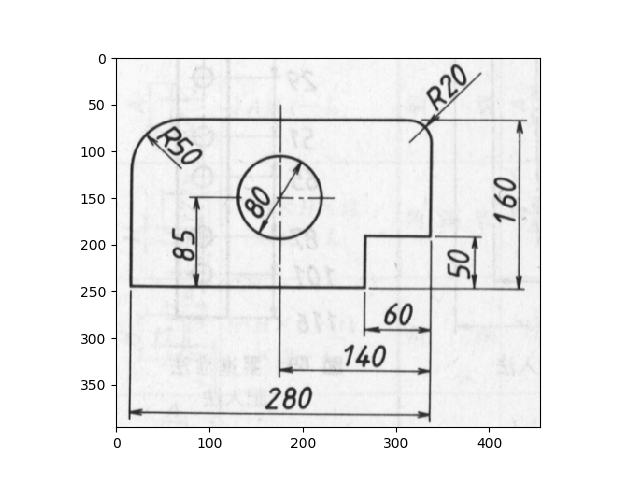
\includegraphics[width = 5cm]{pic/kadai5.png}
        \caption{二値化前の画像}
        \label{beforedivide}
      \end{center}
    \end{minipage}

    \begin{minipage}{0.5\hsize}
      \begin{center}
        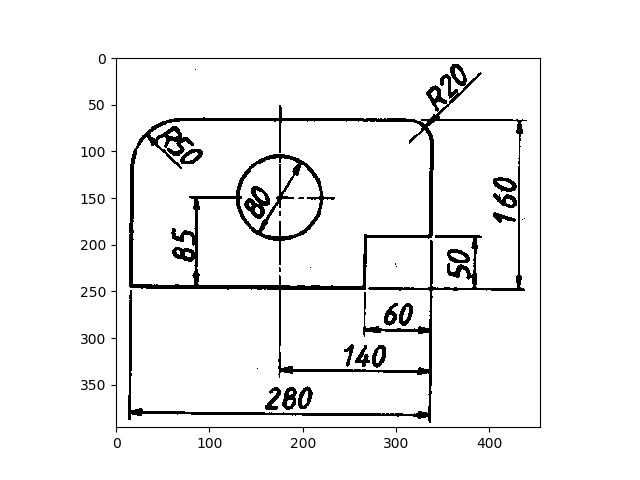
\includegraphics[width = 5cm]{pic/kadai5_200.png}
        \caption{二値化後の画像}
        \label{afterdivide}
      \end{center}
    \end{minipage}
  \end{tabular}
\end{figure}

二値化前の画像(図\ref{beforedivide}) では黒いくすみや消しの残しのような跡が目立っており, 図面が若干見づらくなっているが,
二値化後の画像(図\ref{afterdivide})を比較するとくすみや消しの残しがなくなっており, 字や線も濃くなり, 見やすく処理できていることがわかる.
ヒストグラムから, ノイズが画素値40〜210に分布すると考えたため, 閾値を200にして実装したが,
閾値を210の方向に移動させてやることでよりノイズを除去できる可能性が考えられる.
また, 今回の実験では処理対象が図面であり白と黒のみで色を分けたが, 濃淡のある絵画などに同様の処理を施す場合には,
閾値を複数指定し, 区分ごとに別の画素値を指定してやることで, 三値化, 四値化$\dots$とより詳細で多様な表現ができると思われる.

\subsection{課題6: ヒストグラムと階調変換}
実行した結果を以下に示す.
\begin{figure}[H]
  \begin{tabular}{cc}
    \begin{minipage}{0.5\hsize}
      \begin{center}
        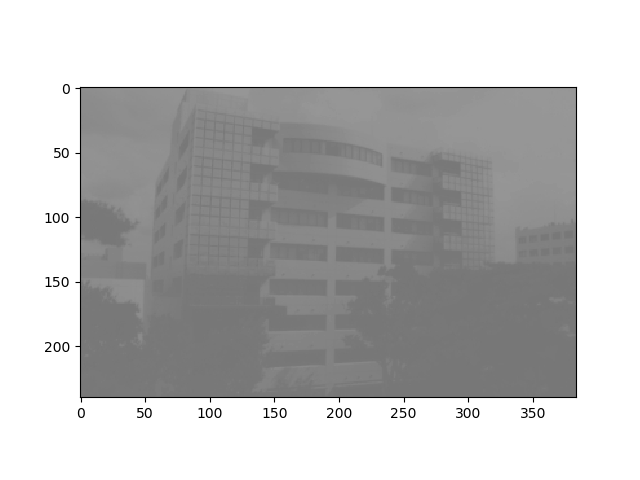
\includegraphics[width = 5cm]{pic/kadai6.png}
        \caption{階調変換前}
        \label{beforevivid}
      \end{center}
    \end{minipage}

    \begin{minipage}{0.5\hsize}
      \begin{center}
        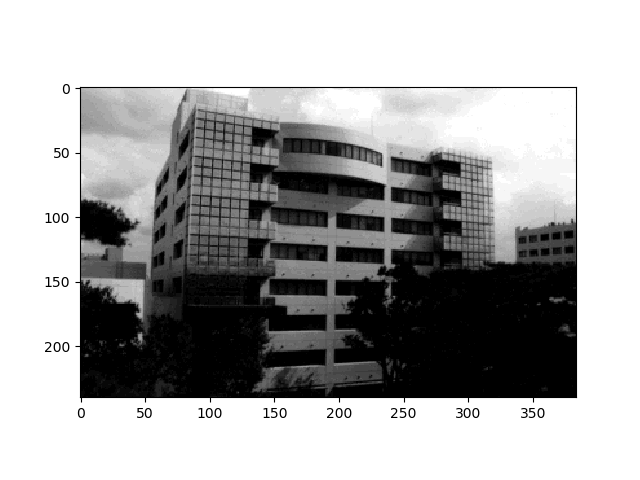
\includegraphics[width = 5cm]{pic/kadai6pic.png}
        \caption{階調変換後}
        \label{aftervivid}
      \end{center}
    \end{minipage}
  \end{tabular}
\end{figure}

\begin{figure}[H]
  \begin{tabular}{cc}
    \begin{minipage}{0.5\hsize}
      \begin{center}
        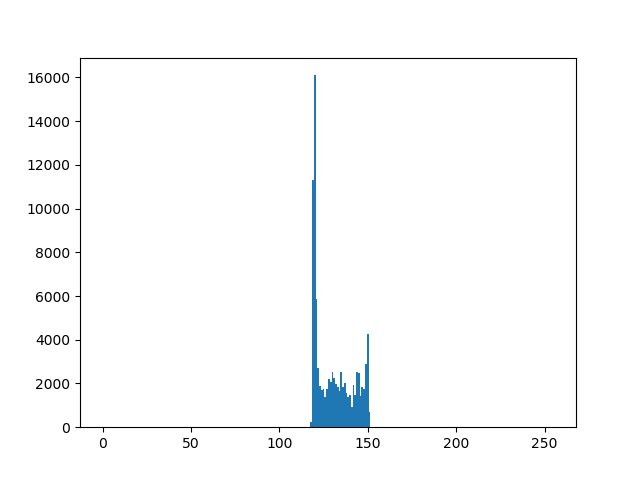
\includegraphics[width = 5cm]{pic/kadai6hist1.png}
        \caption{階調変換前のヒストグラム}
        \label{beforevividhist}
      \end{center}
    \end{minipage}

    \begin{minipage}{0.5\hsize}
      \begin{center}
        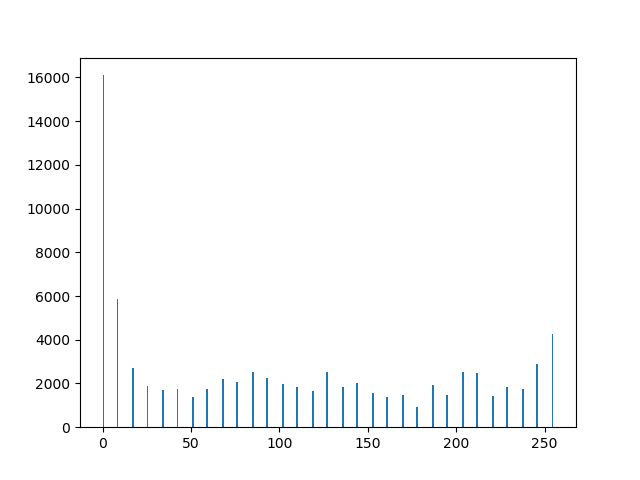
\includegraphics[width = 5cm]{pic/kadai6hist2.png}
        \caption{階調変換後のヒストグラム}
        \label{aftervividhist}
      \end{center}
    \end{minipage}
  \end{tabular}
\end{figure}

階調変換前の画像(図\ref{beforevivid})と階調変換後の画像(\ref{aftervivid})を比較すると,
光の陰影や建物と空の境界が確かに鮮明に変化していることがわかる. ヒストグラムを見ると,
階調変換前(図\ref{beforevividhist})では階調値の分布は120〜150であるが階調変換後(図\ref{aftervividhist})では
階調変換前の階調値分布が0〜255に引き伸ばされた分布になっていることがわかる.
建物や空については鮮明に処理できているものの, 木や影が密集している部分では, 境界や色が識別しづらくなっていることが課題である.
変換後のヒストグラムを見ると,0〜150の範囲の方が150〜255の 範囲よりも同じ画素値が密集していることから,
分布を255の方向にずらすような処理を実装すればさらに鮮明な階調変換が行えると思われる.

\subsection{課題7: 図形の面積の計算}
実行した結果を以下に示す.
\begin{lstlisting}[basicstyle=\ttfamily\footnotesize]
三角形の面積:8145
四角形の面積:9185
五角形の面積:9425
六角形の面積:9545
星形の面積:9265
楕円の面積:9841
\end{lstlisting}
上記のような結果になり, 目視では大小すら判断することが難しいものも処理によって簡単に面積が求められることがわかった.それぞれの画素値をヒストグラムから推測し,
画像中の全ての画素値を調べ, 図形の画素値に該当するものがあれば変数を増やしていき, 最終的に各図形の画素数
が求められるというコードを実装した. 今回は地道な方法での実装をしたが, 他にも
\begin{itemize}
  \item 図形を切り抜いてから255以外の画素数を調べる.
  \item 画素数の範囲を指定し, 該当する画素数を調べる.
\end{itemize}
などの方法が考えられる. また, 調べる画素値の範囲を変更することで, 三角形と四角形の面積の和を求めるといったような
処理も応用してできると考えられる.

\subsection{課題8: 図形の輪郭線の長さの長さの計算}
実行結果を以下に示す.
\begin{table}[H]
  \begin{center}
    \caption{閾値ごとの輪郭線の和}
    \begin{tabular}{|l|l|l|l|l|l|l|}
      \hline
      閾値  & 240  & 220  & 200  & 160 & 120 & 50  \\ \hline
      輪郭線の和 & 2216 & 1896 & 1416 & 1080 & 760 & 376 \\ \hline
    \end{tabular}
  \end{center}
\end{table}

よって, 各々の図形の輪郭線の長さは次のようになった
\begin{table}[H]
  \begin{center}
    \caption{各図形の輪郭線の長さ}
    \begin{tabular}{|l|l|l|l|l|l|l|}
    \hline
    三角形 & 四角形  & 五角形 & 六角形 & 星型 & 楕円 \\ \hline
    320 & 480 & 336 & 320 & 284 & 376  \\ \hline
    \end{tabular}
  \end{center}
\end{table}

まず,二値化する際に, 画素値が高い図形から順番に消えていくよう閾値を求め,
それぞれの場合の周の和を求めた. 合計の周の和から図形を一つ消した後の合計を引くことで, 消えた図形の輪郭線の長さが
計算できる仕組みを利用した. 以下に処理を行った時の画像を示す.

\begin{figure}[H]
  \begin{tabular}{cc}

    \begin{minipage}{0.5\hsize}
      \begin{center}
        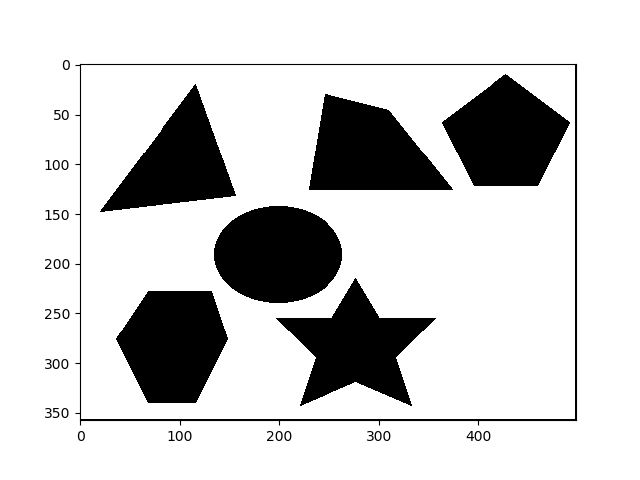
\includegraphics[width = 5cm]{pic/kadai8_2.png}
        \caption{6つ全ての図形の二値化(閾値: 240)}
        \label{all}
      \end{center}
    \end{minipage}

    \begin{minipage}{0.5\hsize}
      \begin{center}
        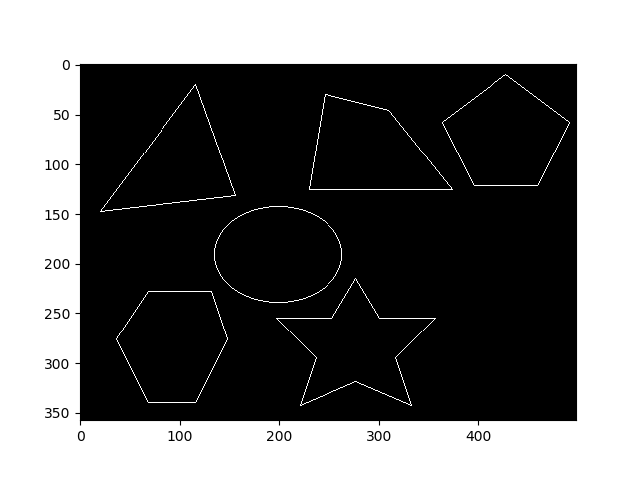
\includegraphics[width = 5cm]{pic/kadai8_3.png}
        \caption{ラプラシアンフィルタ変換後(閾値: 240)}
        \label{all_raplace}
      \end{center}
    \end{minipage}

  \end{tabular}
\end{figure}

\begin{figure}[H]
  \begin{tabular}{cc}

    \begin{minipage}{0.5\hsize}
      \begin{center}
        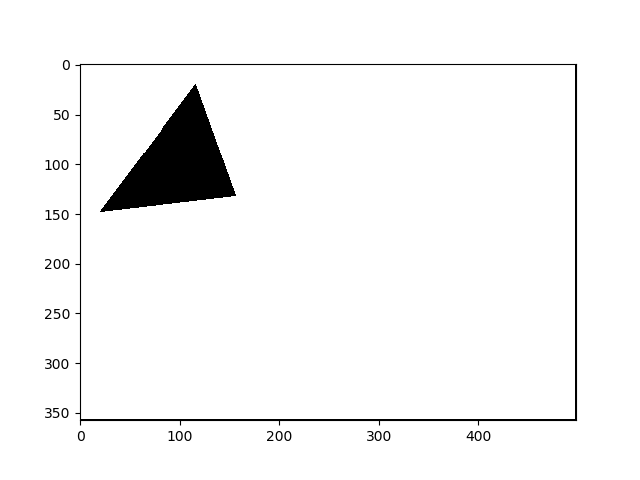
\includegraphics[width = 5cm]{pic/kadai8_5.png}
        \caption{三角形のみ二値化(閾値: 50)}
        \label{triangle}
      \end{center}
    \end{minipage}

    \begin{minipage}{0.5\hsize}
      \begin{center}
        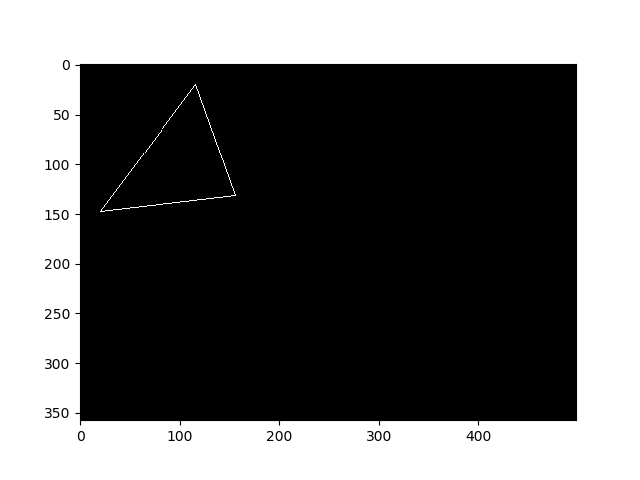
\includegraphics[width = 5cm]{pic/kadai8_4.png}
        \caption{ラプラシアンフィルタ変換後(閾値: 50)}
        \label{tri_raplace}
      \end{center}
    \end{minipage}

  \end{tabular}
\end{figure}

この課題でも地道に検証し, 一つずつ輪郭線の長さを計算するという実装をしたが,
他にも実装の方法が次のように考えられる.
\begin{itemize}
  \item 図形を切り抜いてから一つずつ輪郭線の長さを調べる.
  \item 画素数を調べ, 特定の図形だけを二値化したのちに輪郭線の長さを調べる.
  \item ラプラシアンフィルタを先にかけ, 一つだけ図形が残るよう画素値の範囲を指定したのちに二値化して輪郭線の長さを調べる.
\end{itemize}

なお3つ目のラプラシアンフィルタを先にかけたのちに二値化するという処理を試みたものの, 頂点など, 線と線が重なる点の画素値が線に比べて低くなっており,
特定の画素値の範囲で一つの図形だけを抽出するという操作ができなかった.

\section{結論}
今回の実験では, 基本的なデジタル画像処理を実際に自分で実装する作業を通して, その基本原理と特性について理解することを目的とした.
基本的な画像の取り扱い方, 平滑化フィルタや差分型フィルタを基本とするフィルタリングの技術, 二値化や階調変換からなる点演算を課題1〜6で理解, 実装, 特製の確認を行い, 課題7, 8ではそれらの技術を用いて
複数の図形の面積や輪郭線の長さを求めやすいよう画像処理を施し, 計算した. どの操作も画像処理の基本ではあるが, これらの処理を応用するだけでも行える画像処理は多く存在すると思われる. 現代では画像処理の技術はスマートフォン, カメラ, ロボットと当たり前かつ広く使用されているものであり,
生活, あるいは製品開発の開発をする上で切っても切れない存在である. その技術を実際に原理から学び, 実装することは技術者としても一人の人間としても大切な経験であり, これからも積極的に挑戦していきたい.
\section{参考文献}
[1]知能機械工学基礎実験,電気通信大学  知能機械工学科
\end{document}
